\chapter{実装回路図ならびにPCBレイアウト図}
実装した送受信回路の回路図ならびにPCBレイアウト図を次頁以降に添付する.

\begin{landscape}
\begin{figure}[p]
\begin{center}

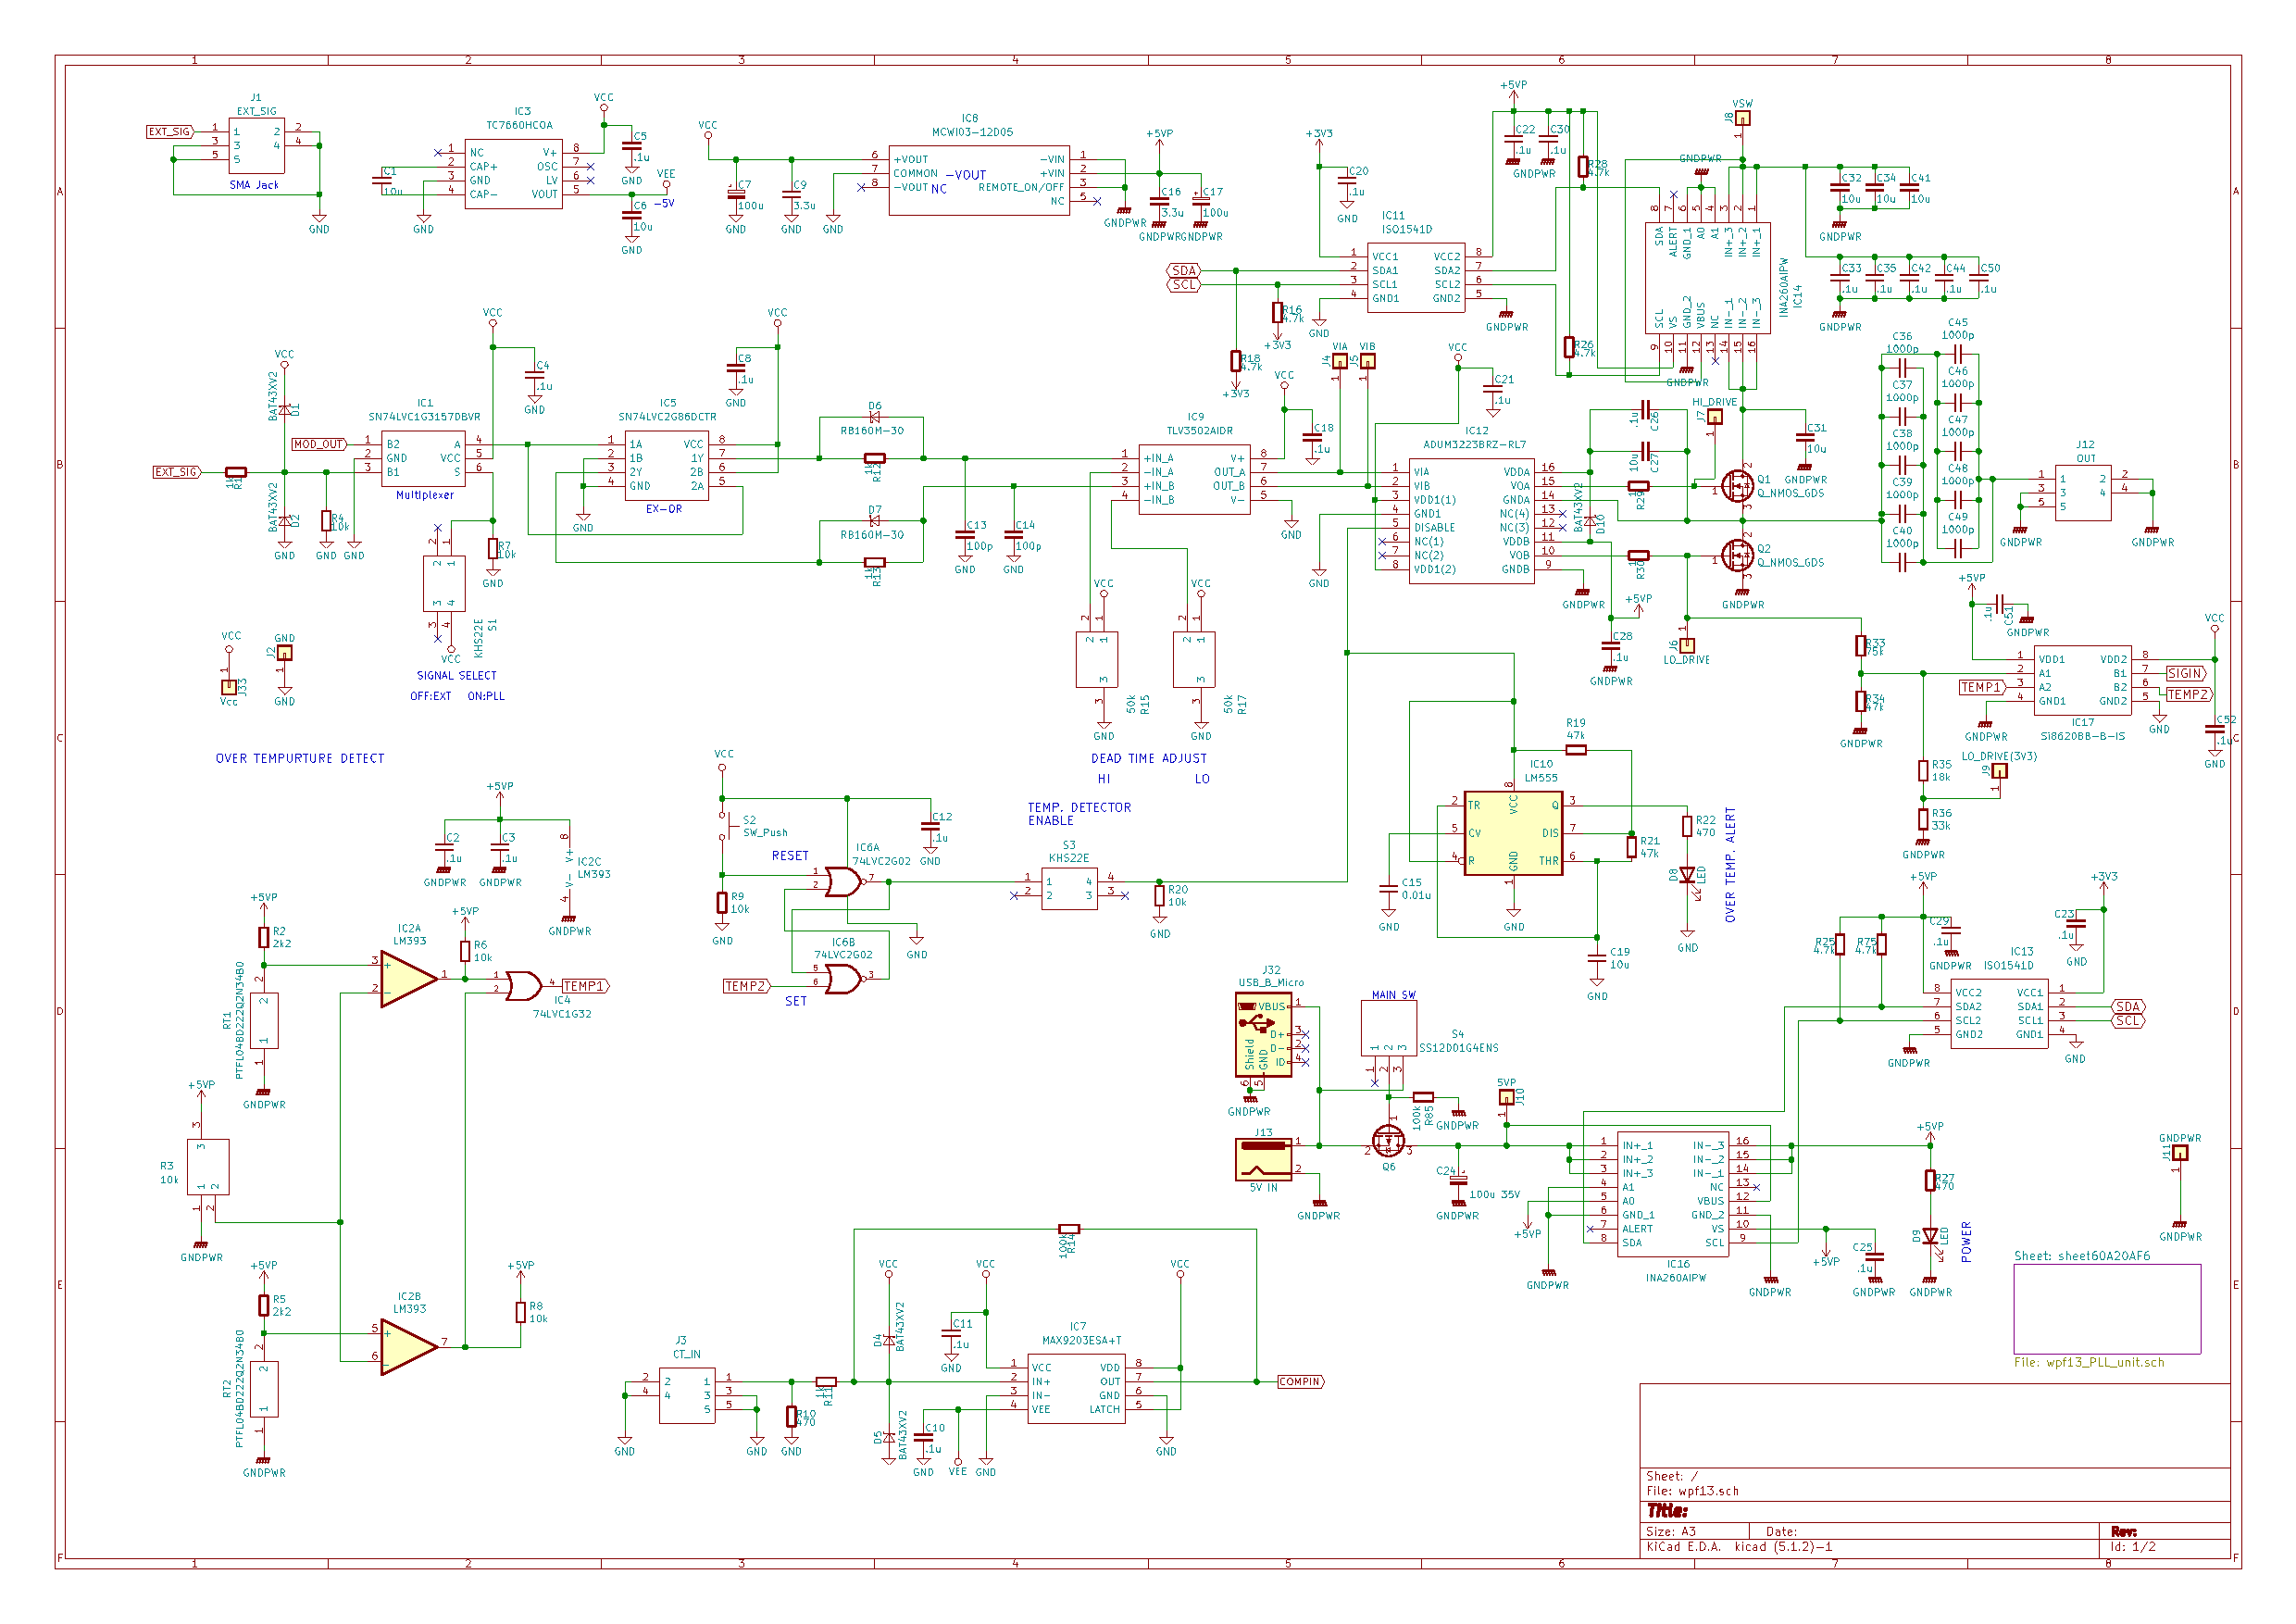
\includegraphics[width=220mm]{figures/wpf13_circuit1.pdf}
  \caption{送信側回路図(1/2)}

  \end{center}
\end{figure}
\end{landscape}


\begin{landscape}
\begin{figure}[p]
\begin{center}

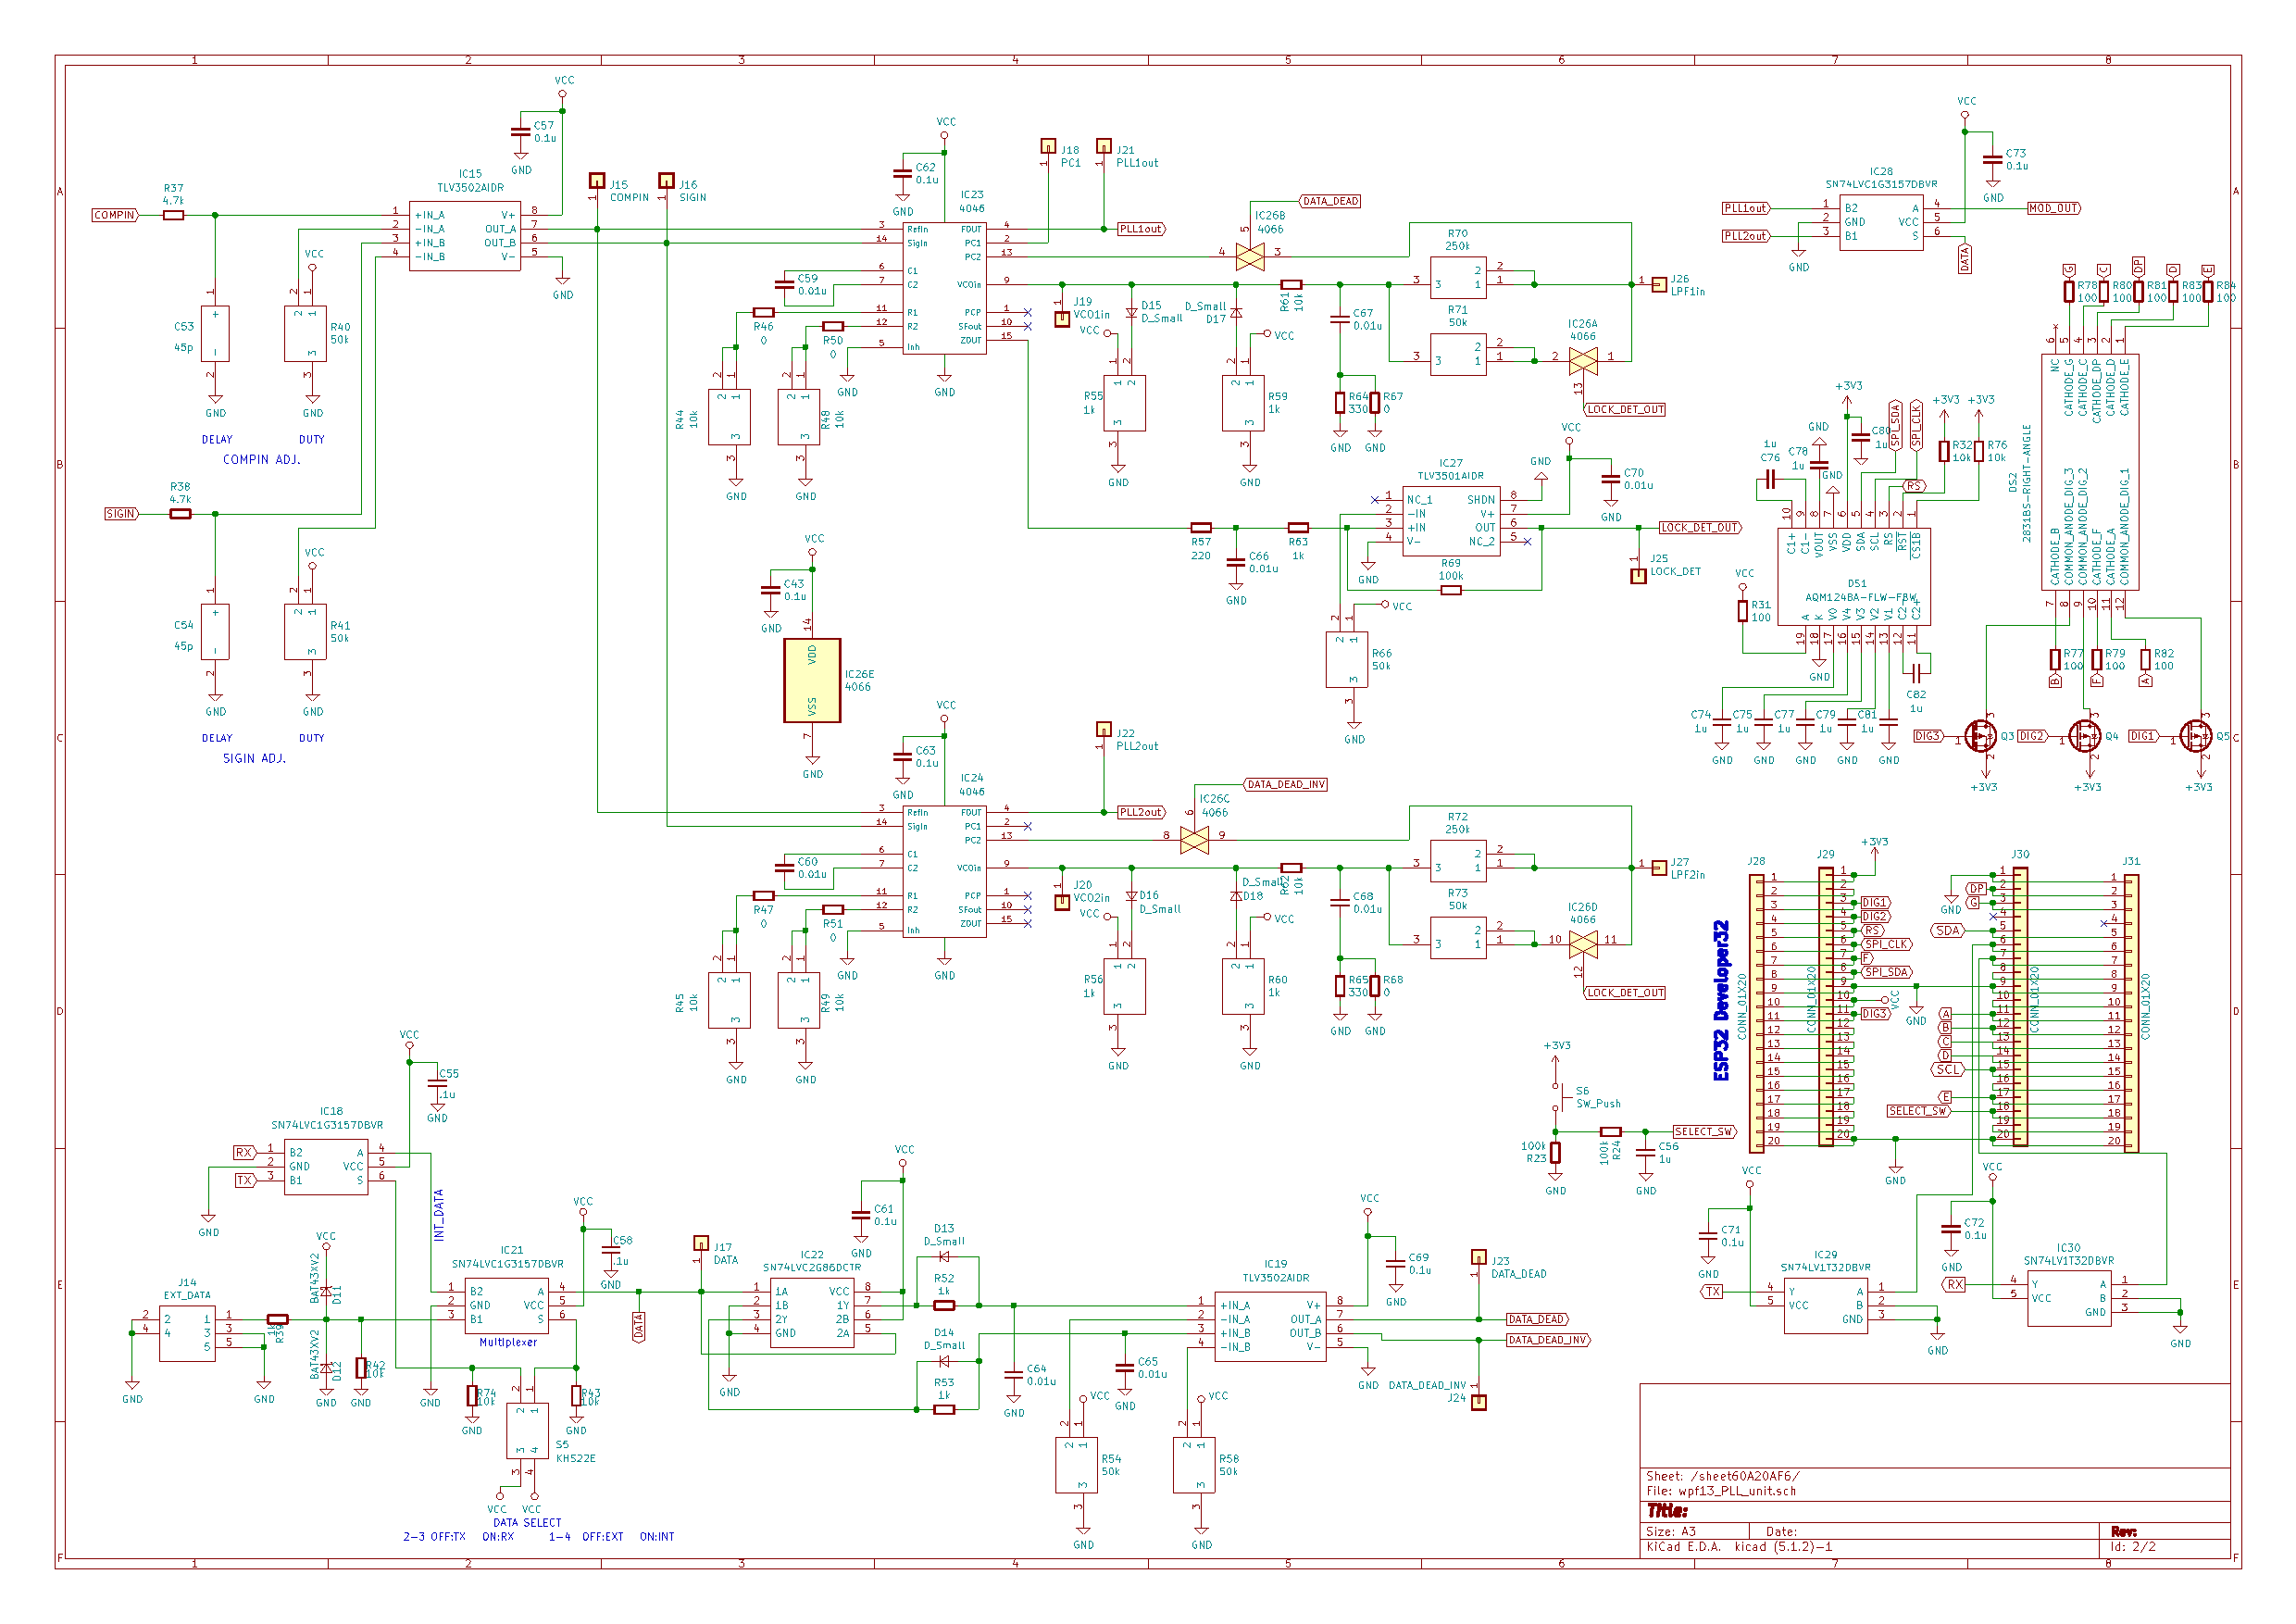
\includegraphics[width=220mm]{figures/wpf13_circuit2.pdf}
  \caption{送信側回路図(2/2)}

  \end{center}
\end{figure}
\end{landscape}


\begin{landscape}
\begin{figure}[p]
\begin{center}

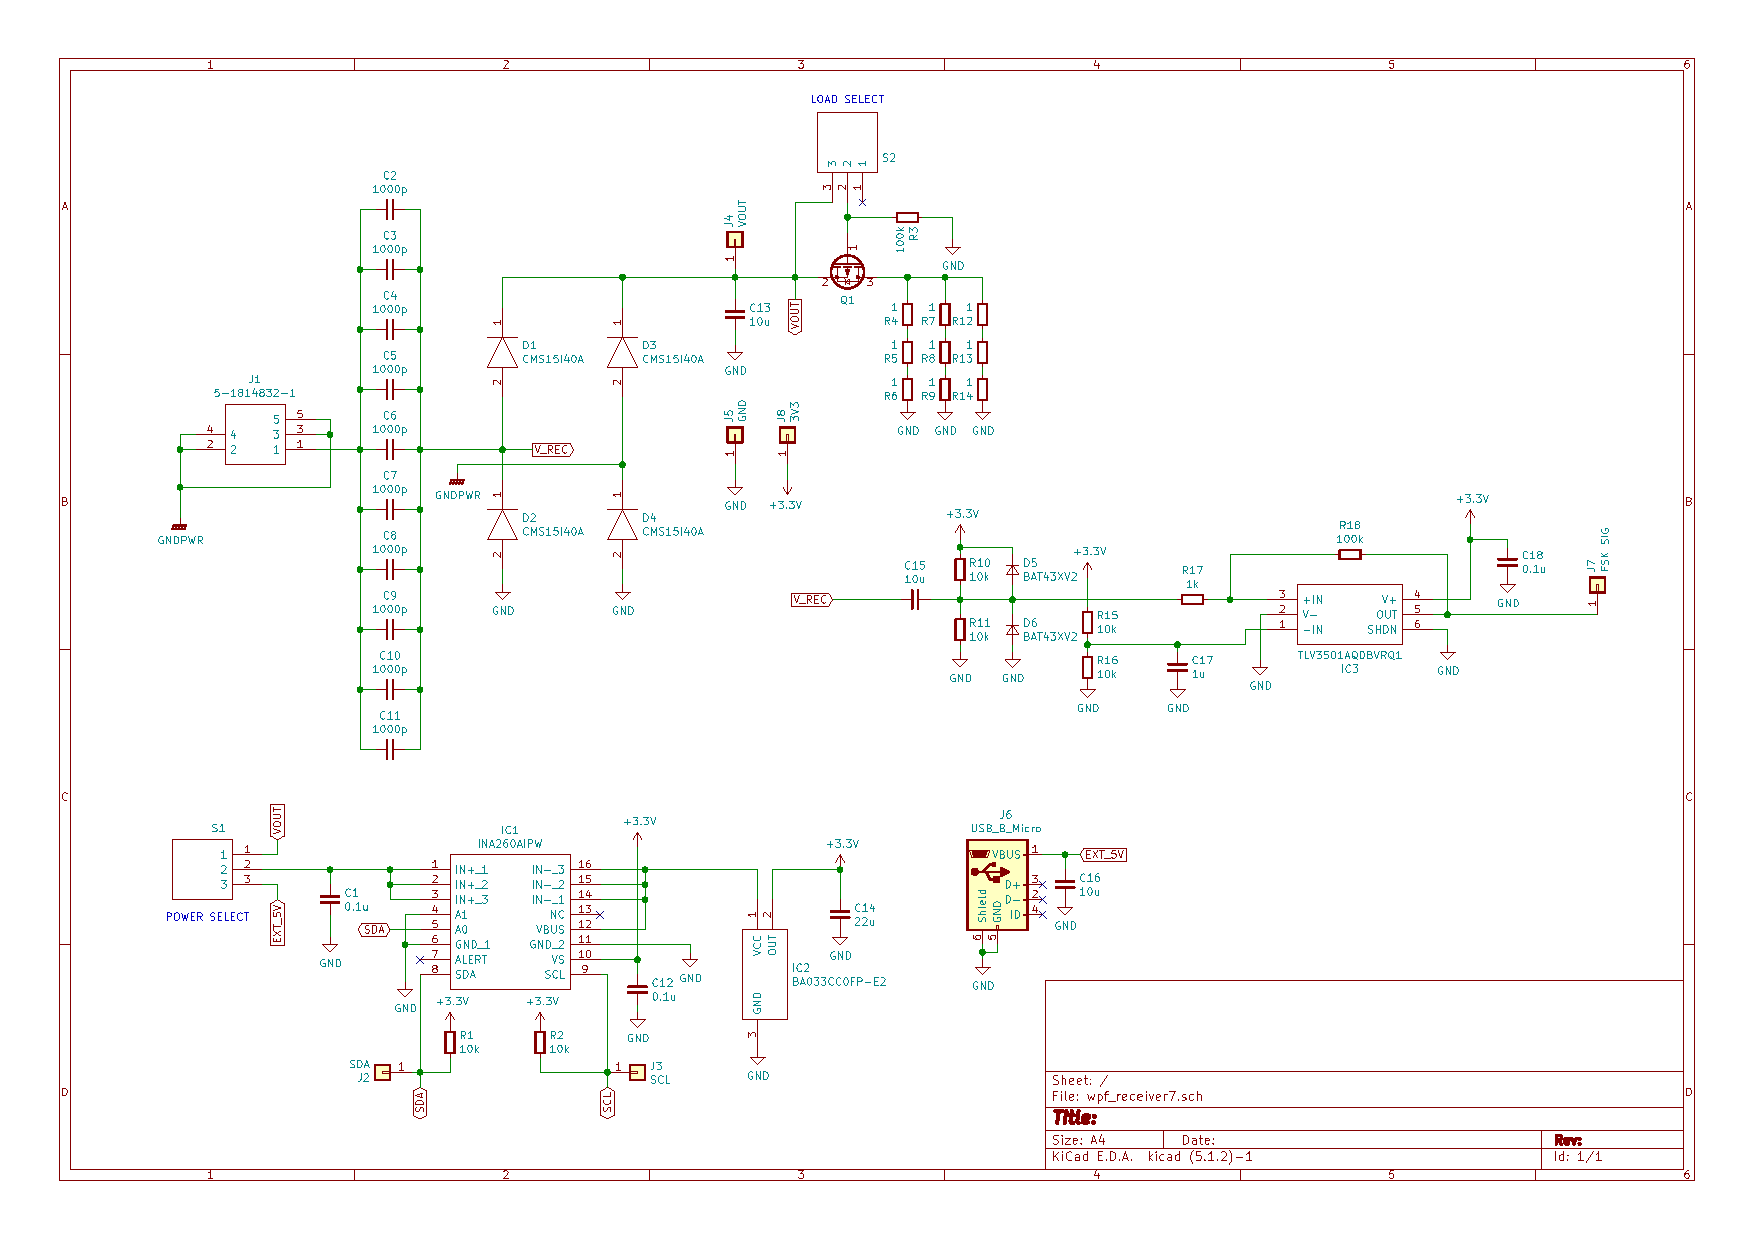
\includegraphics[width=220mm]{figures/wpf_receiver7_circuit.pdf}
  \caption{受信側回路図}

  \end{center}
\end{figure}
\end{landscape}


\begin{figure}[p]

	\begin{center}
    \subfloat[表面]{
    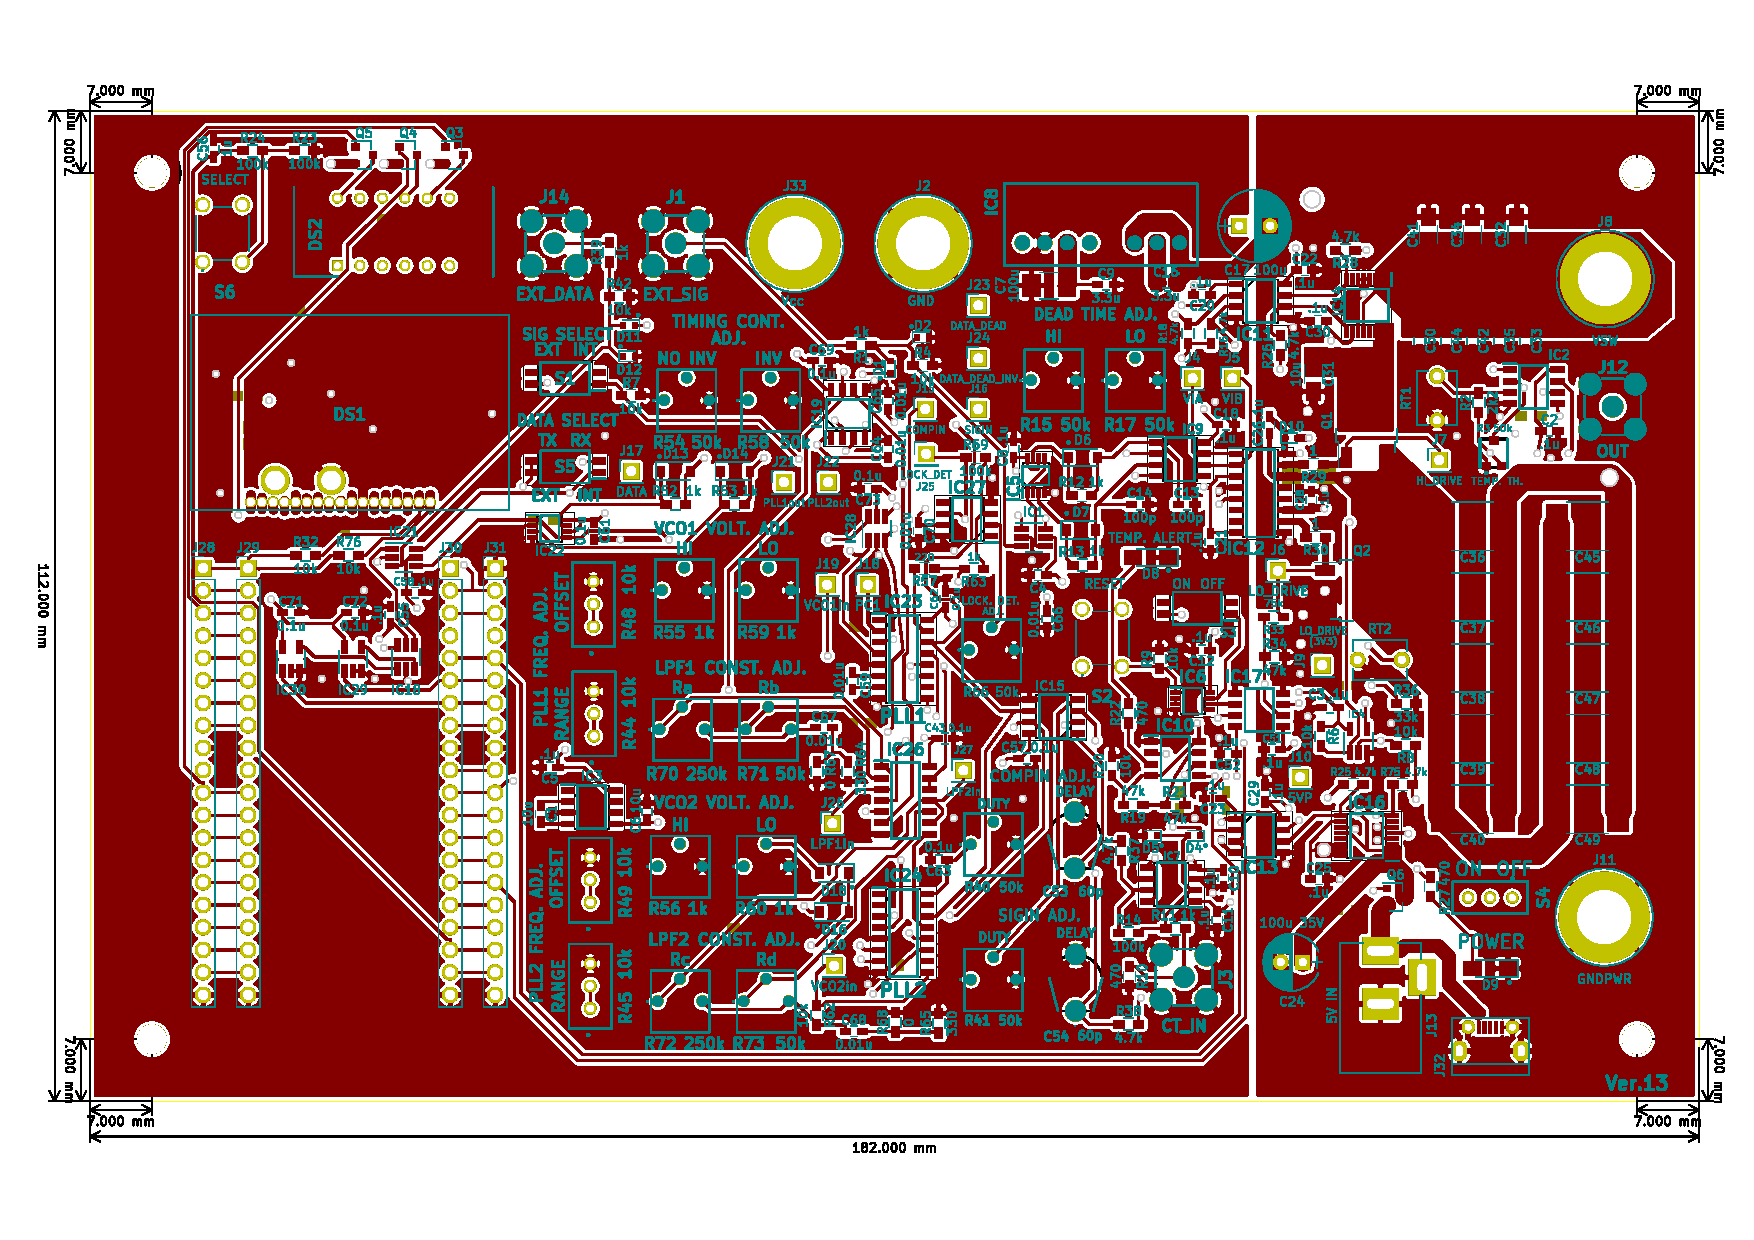
\includegraphics[width=150mm]{figures/wpf13_board_002.pdf}
    }
    \\ 
    \subfloat[内層1面]{
    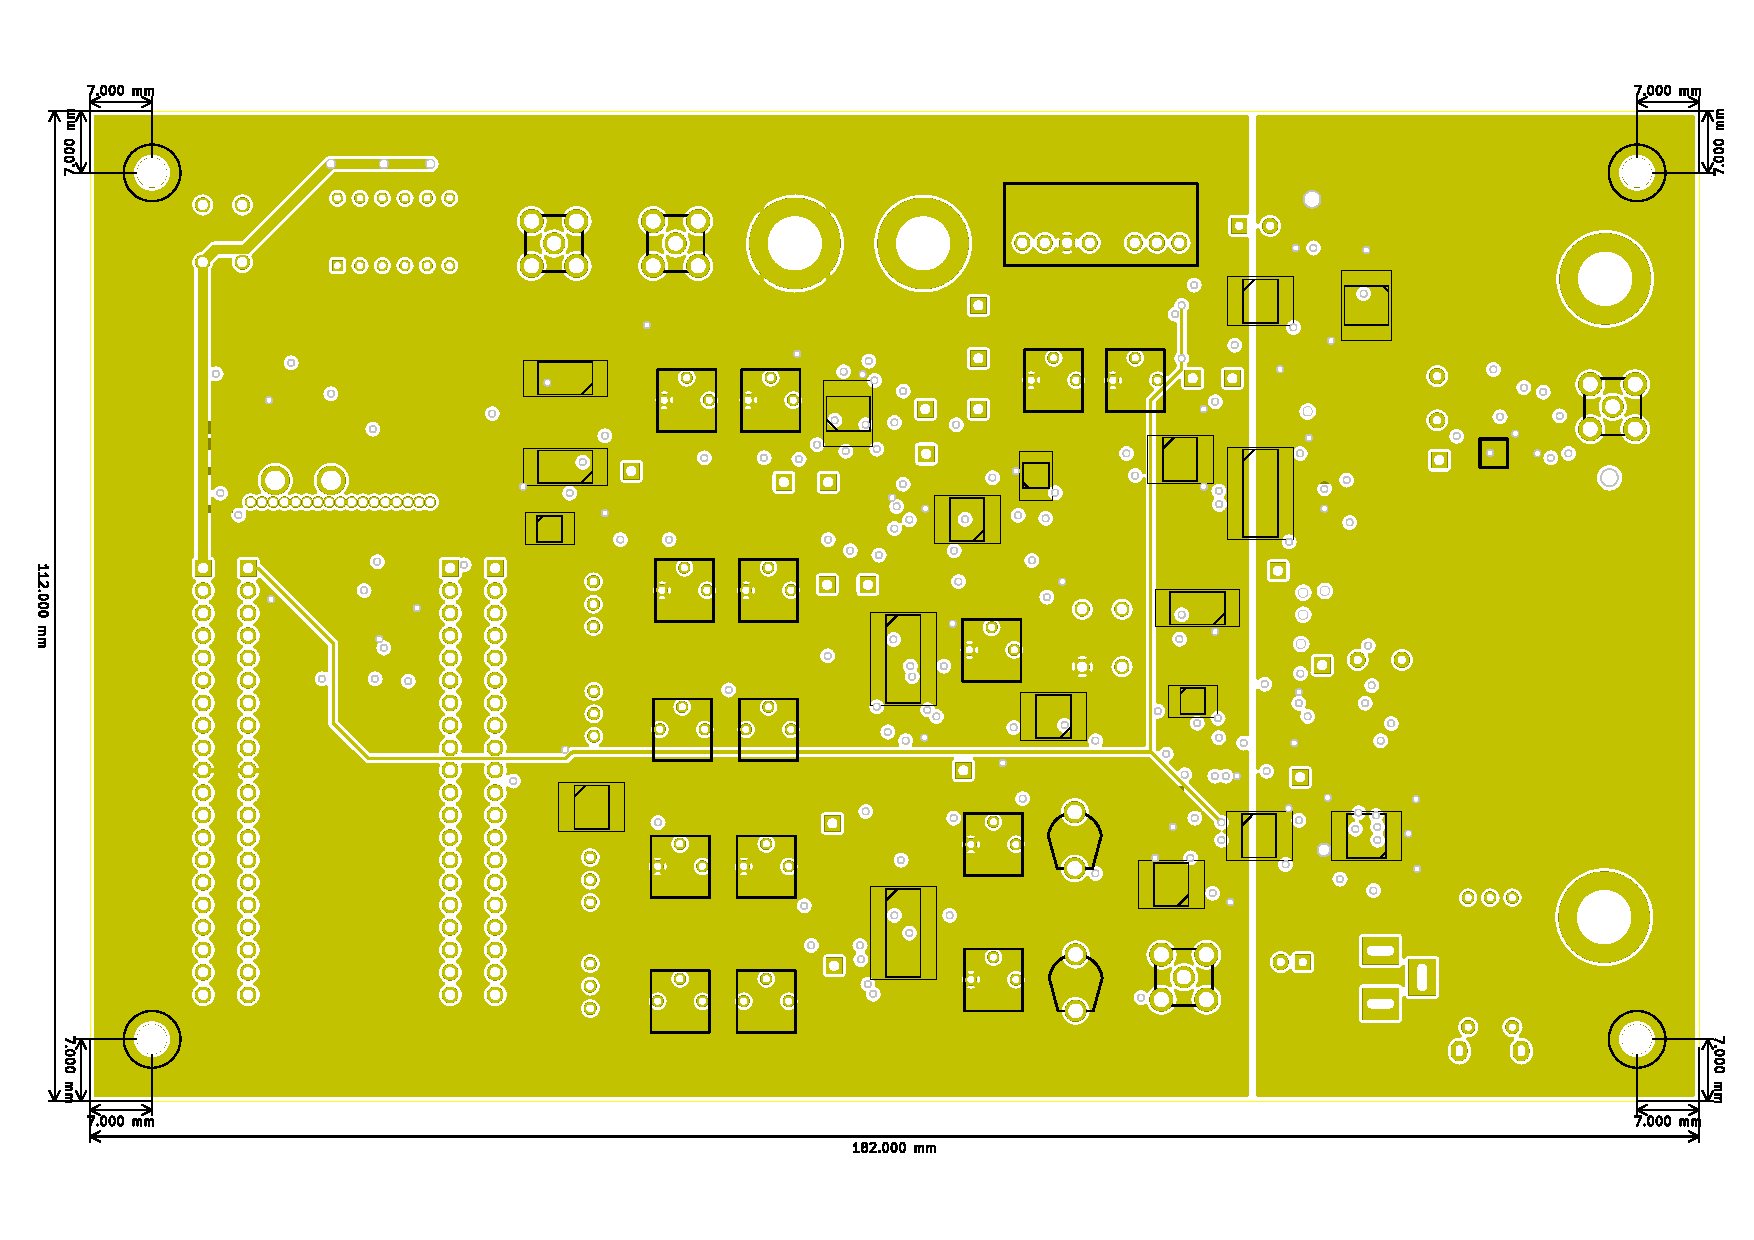
\includegraphics[width=150mm]{figures/wpf13_board_003.pdf}
    }
    \\ 
  \end{center}
\end{figure}

\begin{figure}[p]
	\begin{center}
    
    \setcounter{subfigure}{2}
    
    \subfloat[内層2面]{
    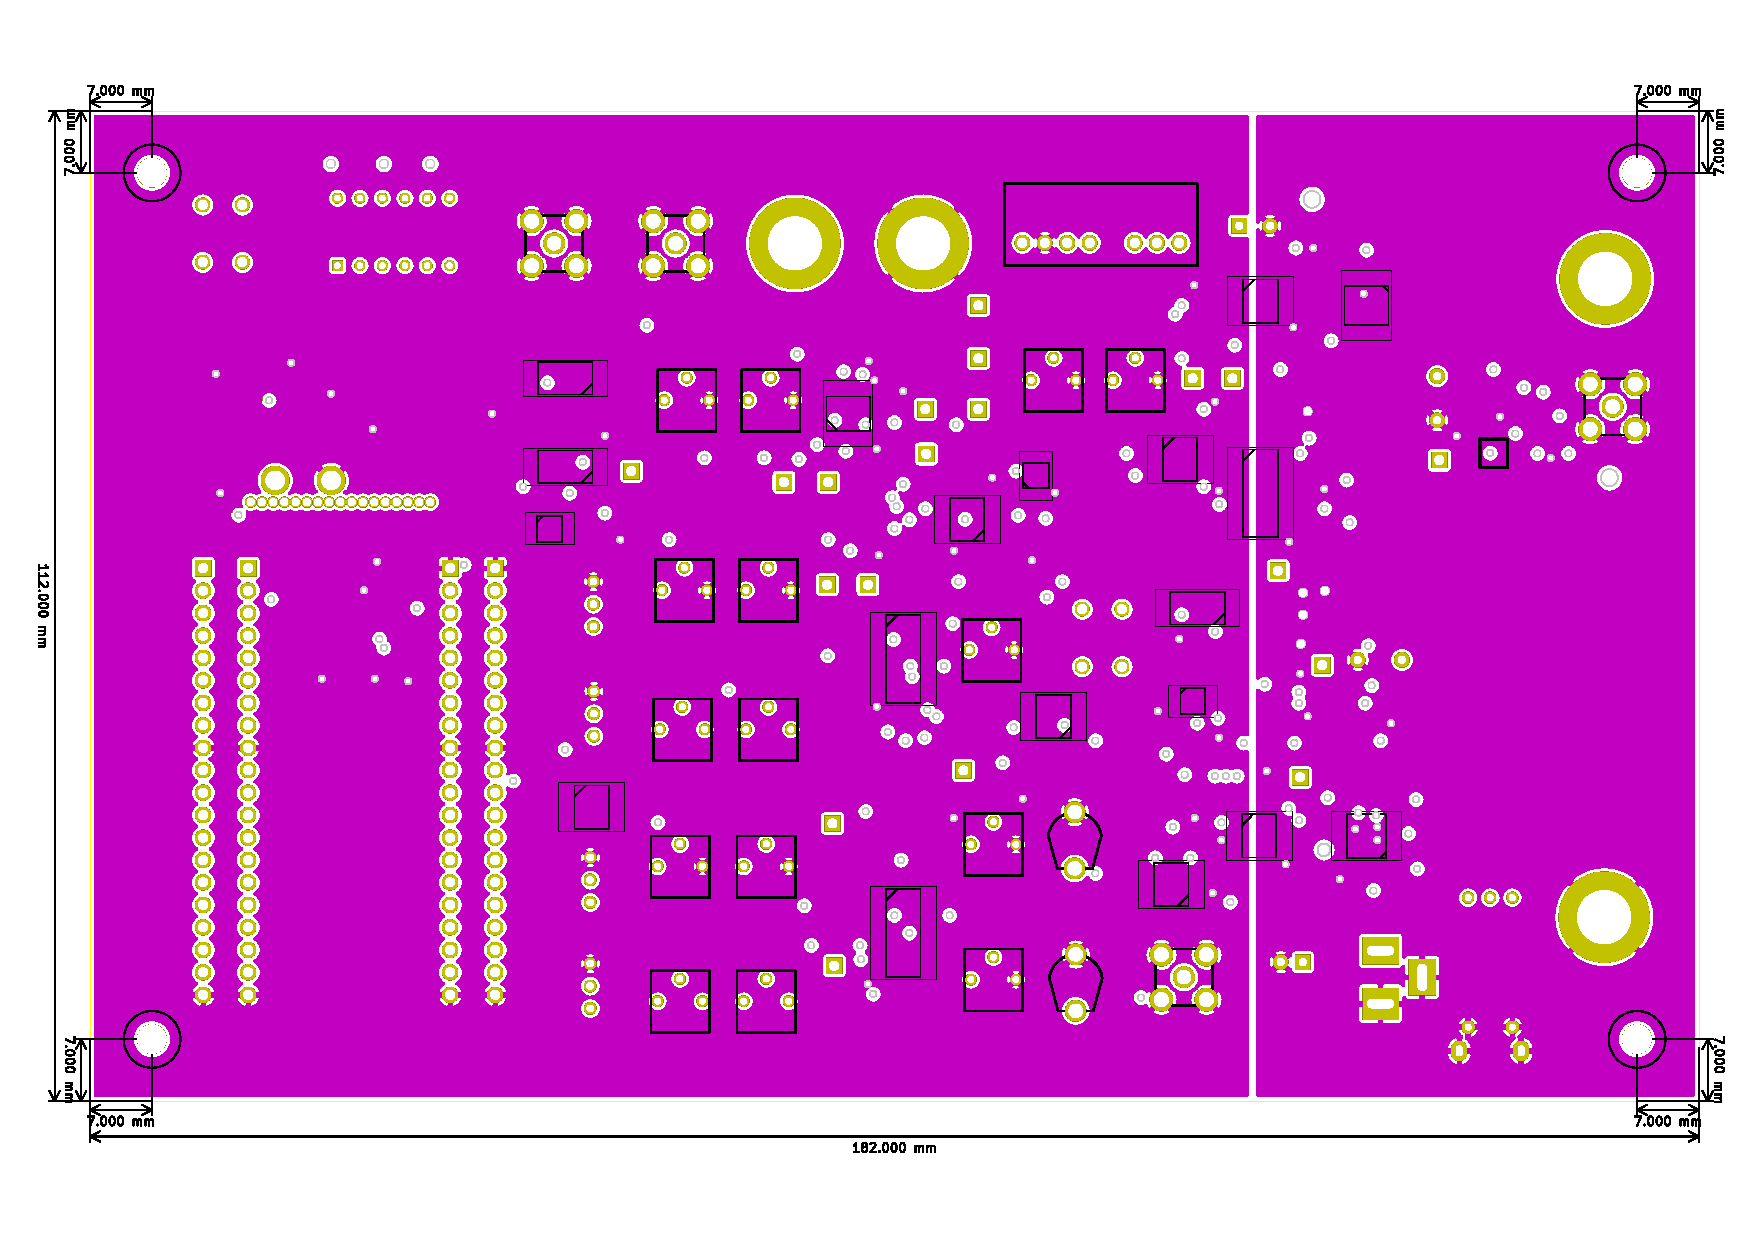
\includegraphics[width=150mm]{figures/wpf13_board_004.pdf}
    }
    \\ 
   
    \subfloat[裏面]{
    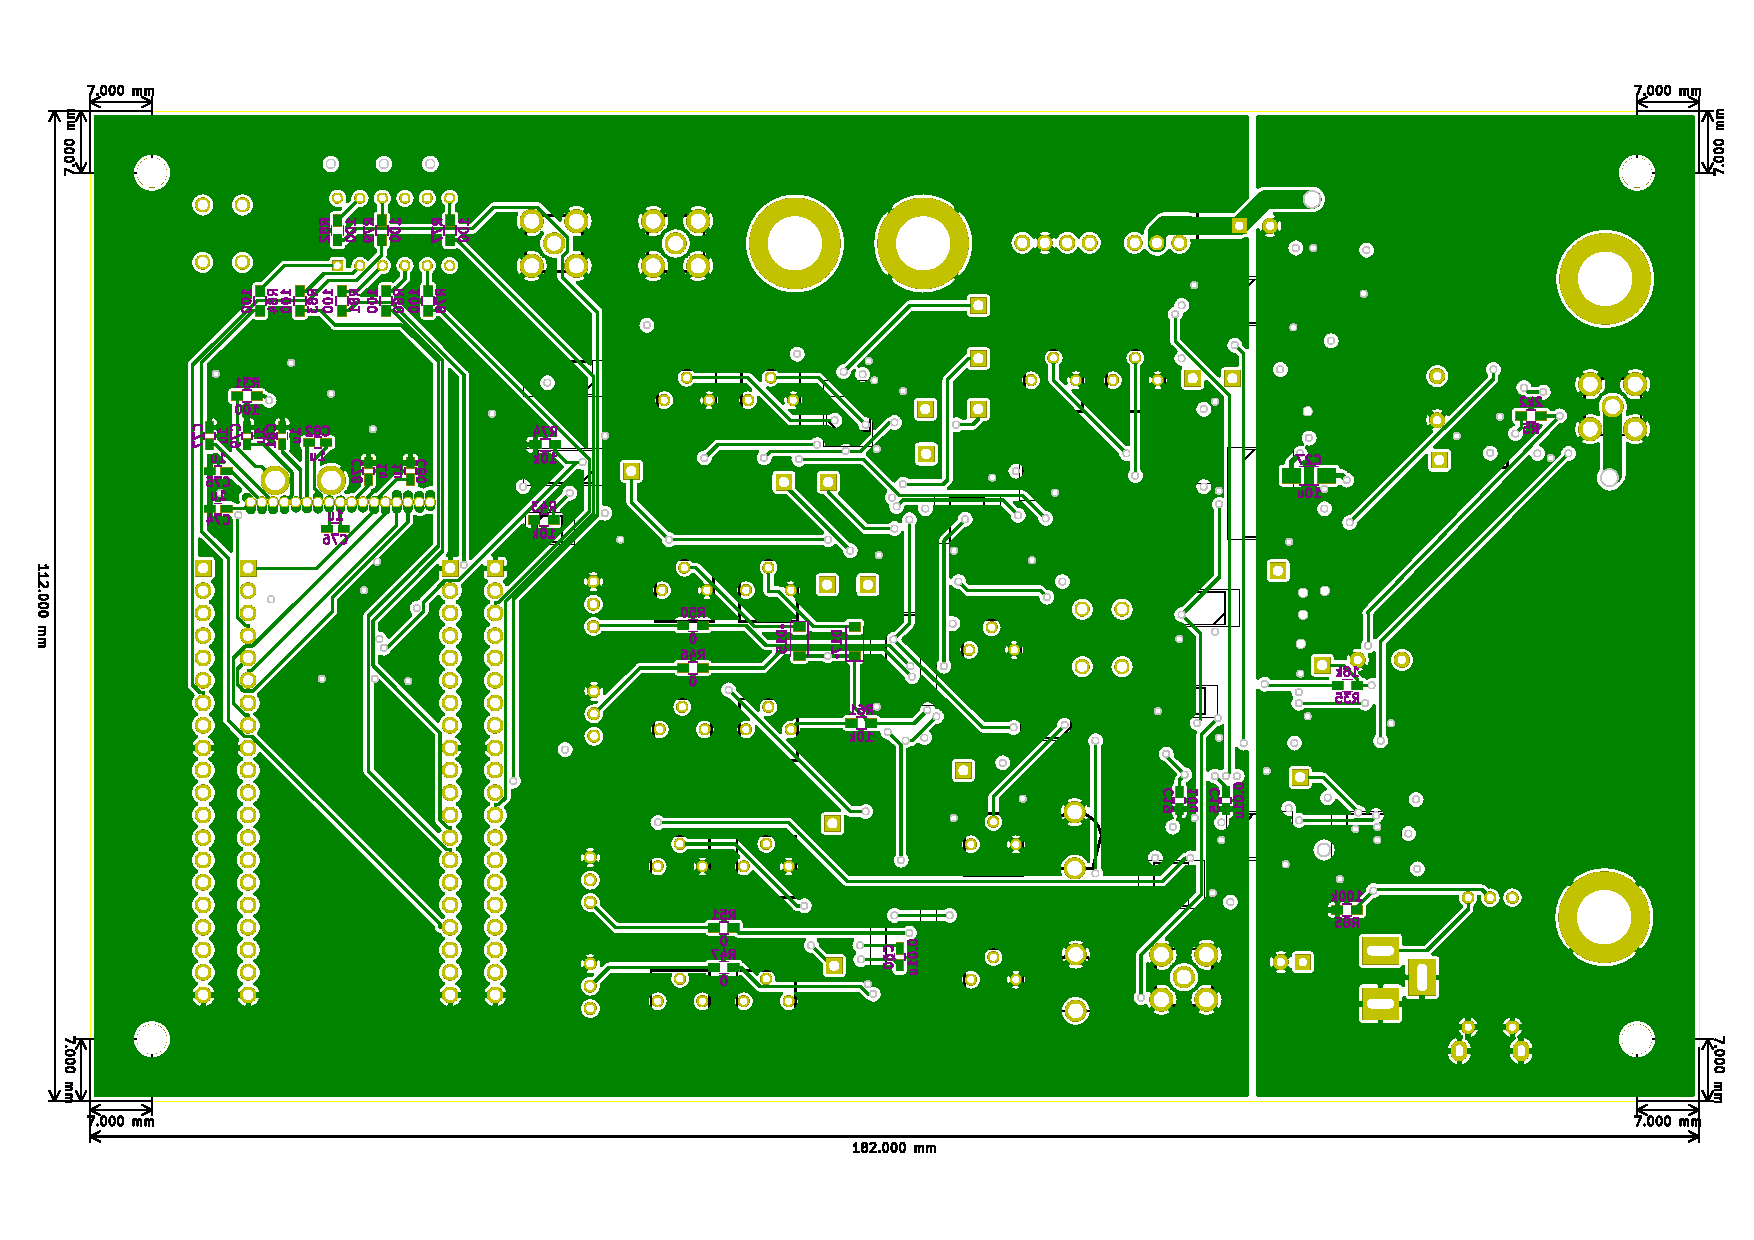
\includegraphics[width=150mm]{figures/wpf13_board_005.pdf}
    }

  \caption{送信側PCBレイアウト図}

    \end{center}
\end{figure}
  
  \begin{figure}[p]

	\begin{center}
    \subfloat[表面]{
    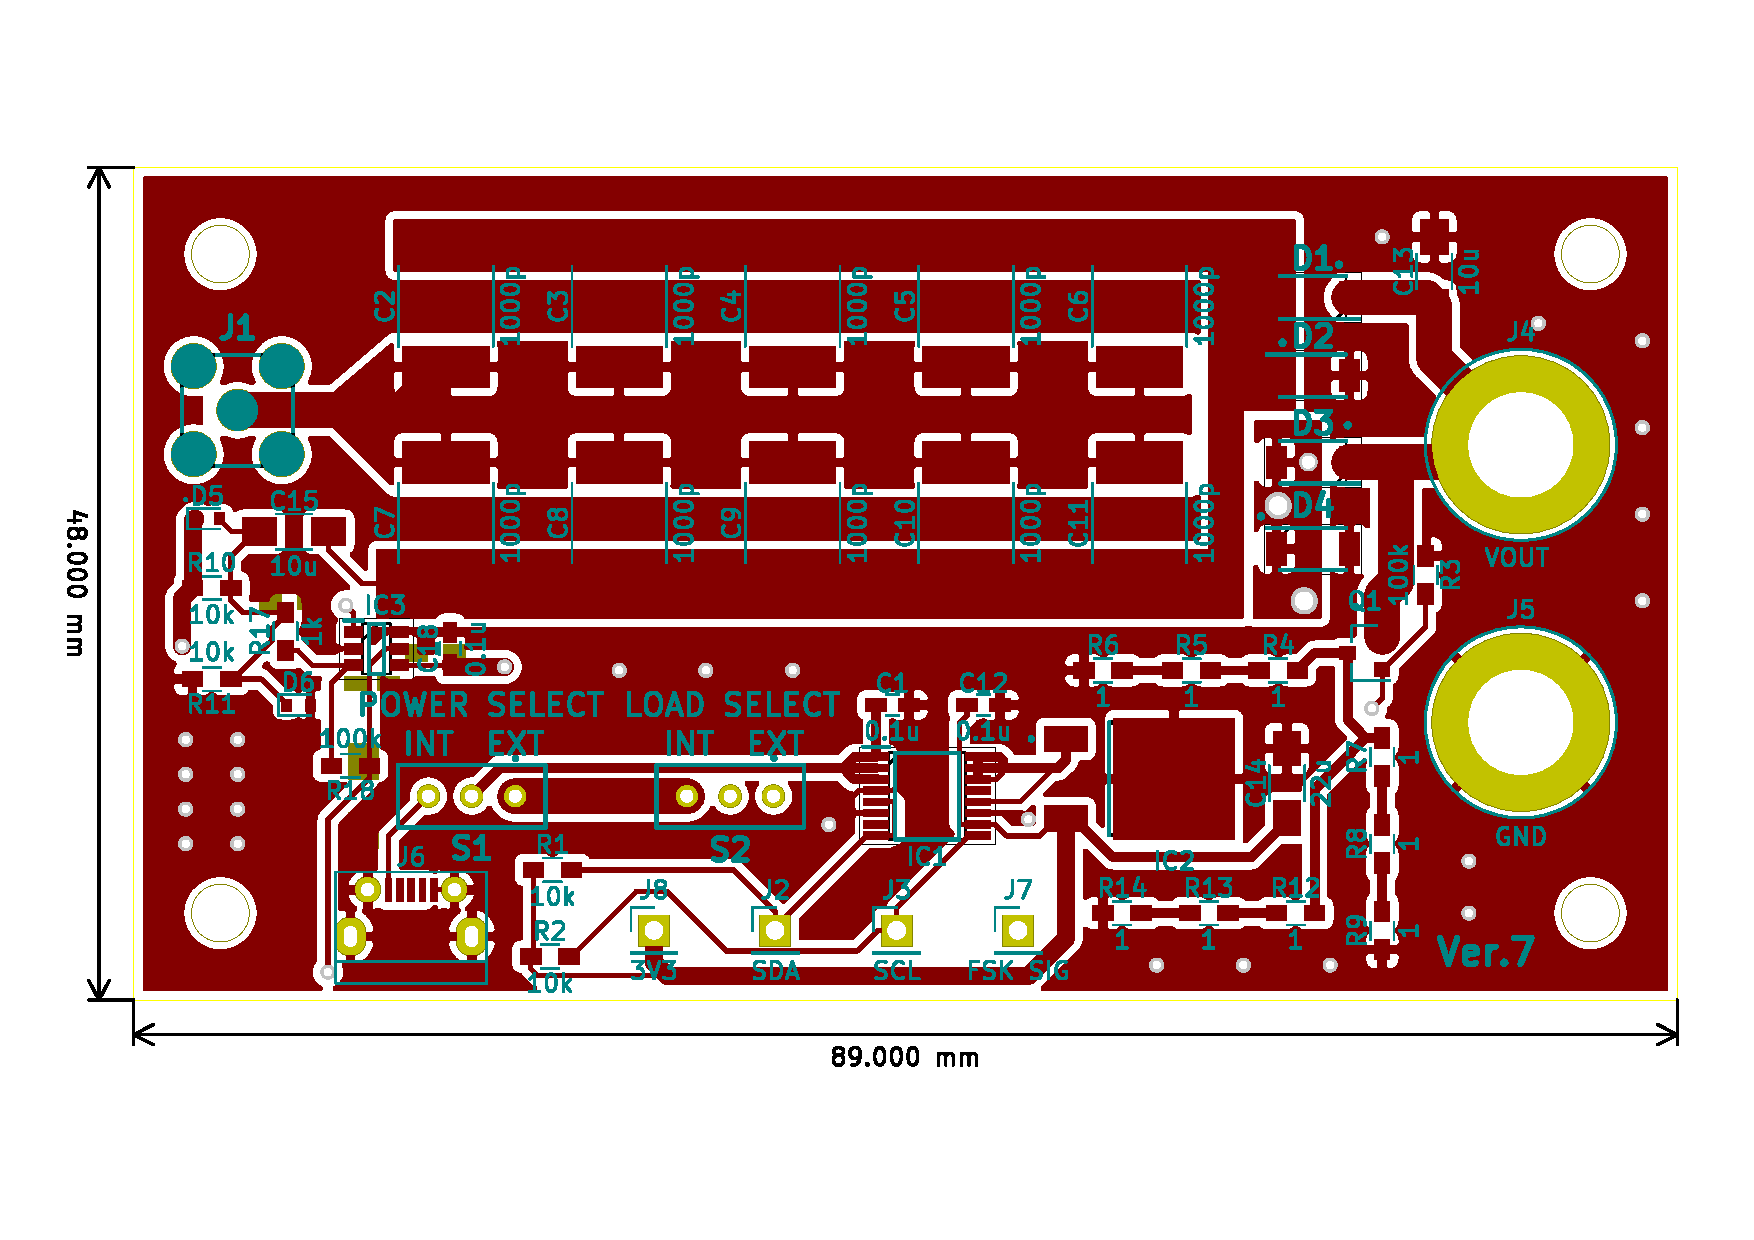
\includegraphics[width=150mm]{figures/wpf_receiver7_board_002.pdf}
    }
    \\ 
    \vspace{5mm}
    \subfloat[裏面]{
    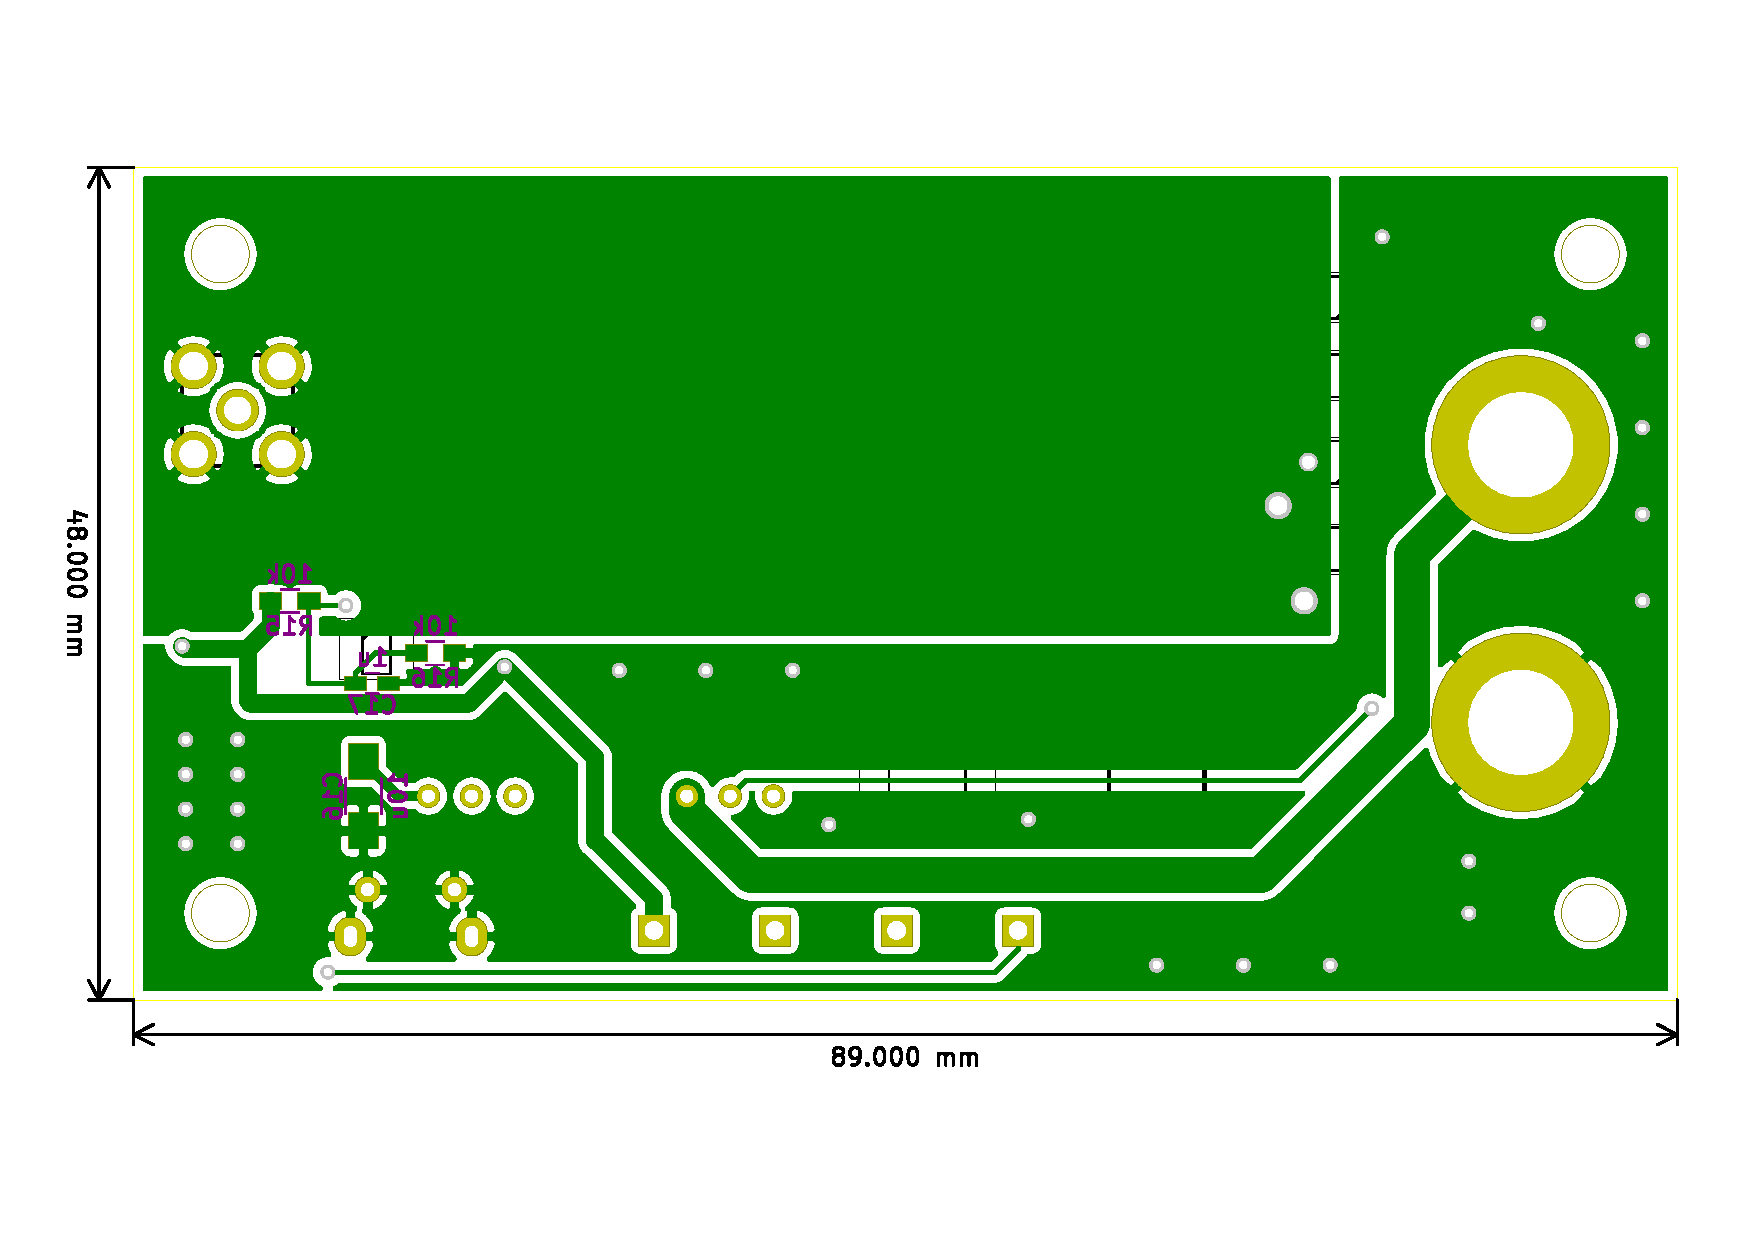
\includegraphics[width=150mm]{figures/wpf_receiver7_board_003.pdf}
    }
    \\ 
    \caption{受信側PCBレイアウト図}
  \end{center}
\end{figure}

\chapter{FSK復調器のVerilog-HDLソースコード}
FPGAを用いたFSK復調器のVerilog-HDLソースコードならびに論理シミュレーション用テストベンチを以下に示す.

\begin{lstlisting}[caption=FSK復調器]

module counter7_for_thesis(
    input clk,
    input serial_datain, 
    input sw0,
    input sw1,
    input sw2,
    input sw3,
    input btn0,
    input extfsksig, //b10
    
    output serial_dataout,
    output led0,
    output b1,
    output b2,
    output b3,
    output b4,
    output b7,
    output b8,
    output b9
        );  


parameter low_freq=598; /*kHzで指定*/  
parameter high_freq=979;
parameter integer cnt_fspace=(1/(low_freq*2*0.000008));
parameter integer cnt_fmark=(1/(high_freq*2*0.000008));  
parameter integer threshold=167;

reg [19:0] cntdata=20'd0;
reg [31:0] cntfspace=32'd0;
reg [31:0] cntfmark=32'd0;
reg [31:0] demodcnt_1p=32'd0;
reg [31:0] demodcnt_2p=32'd0;
reg [31:0] demodcnt_p=32'd0;
reg [31:0] difference_p=32'd0;
reg [31:0] bps=32'd0;
reg [31:0] rstpls_p=32'b0;
reg [63:0] resetcounter=64'd0; 

reg fmark=1'b0; /* high freq*/
reg fspace=1'b0; /*low freq*/
reg fsksig=1'b0;
reg fdata=1'b0;
reg datachange=1'b0;
reg demodout=1'b0;
reg cntrst_p=1'b0;    
reg resetflag=1'b0;
reg sigselect=1'b0;
reg recoverflag=1'b0;

initial @(negedge demodout) recoverflag<=1'b1;

always @(posedge clk)begin


/* set rate of pseudo data */
/////////////////////////////////////////////////////
       
         if(sw3==0 & sw2==0 & sw1==0& sw0==0) bps<='d300;
    else if(sw3==0 & sw2==0 & sw1==0& sw0==1) bps<='d600;
    else if(sw3==0 & sw2==0 & sw1==1& sw0==0) bps<='d1200;
    else if(sw3==0 & sw2==0 & sw1==1& sw0==1) bps<='d2400;
    else if(sw3==0 & sw2==1 & sw1==0& sw0==0) bps<='d4800;
    else if(sw3==0 & sw2==1 & sw1==0& sw0==1) bps<='d9600;
    else if(sw3==0 & sw2==1 & sw1==1& sw0==0) bps<='d14400;
    else if(sw3==0 & sw2==1 & sw1==1& sw0==1) bps<='d19200;
    else if(sw3==1 & sw2==0 & sw1==0& sw0==0) bps<='d38400;
    else if(sw3==1 & sw2==0 & sw1==0& sw0==1) bps<='d57600;
    else if(sw3==1 & sw2==0 & sw1==1& sw0==0) bps<='d115200;
    else if(sw3==1 & sw2==0 & sw1==1& sw0==1) bps<='d230400;
    else if(sw3==1 & sw2==1 & sw1==0& sw0==0) bps<='d460800;
    else if(sw3==1 & sw2==1 & sw1==0& sw0==1) bps<='d921600;
    else bps<='d115200;
    
/////////////////////////////////////////////////////


/*genarate pseudo FSK signal*/
/////////////////////////////////////////////////////
    if(cntfspace == cnt_fspace) begin
        cntfspace<=32'd0; // reset cnt //
        fspace<=~fspace;
 end
        
else begin
    cntfspace<=cntfspace+32'd1;
 end
 
////////////////////////////////////////////
 
     if(cntfmark == cnt_fmark) begin
        cntfmark<=32'd0; // reset cnt //
        fmark<=~fmark;
 end
        
else begin
    cntfmark<=cntfmark+32'd1;
 end
 
////////////////////////////////////////////

      if(cntdata == 'd125000000/bps) begin
        cntdata<=20'd0; // reset cnt //
       fdata<=~fdata;
 end
        
else begin
    cntdata<=cntdata+20'd1;
 end
 
///////////////////////////////////////////////////// 
  
  
/*choose internal(pseudo) or external FSK signal*/
/////////////////////////////////////////////////////
 
 if(btn0==1) sigselect<=~sigselect;
 
 if(sigselect==0) begin
 
    if(fdata==0)   begin
    fsksig<=fspace;
    end
     else begin
    fsksig<=fmark;
    end
 end
 
 if(sigselect==1) fsksig<=extfsksig;
 
/////////////////////////////////////////////////////


/*generate counter-reset pulse*/
/////////////////////////////////////////////////////

if(fsksig==1'b1) begin  
    rstpls_p<=rstpls_p+1'b1;
        if(rstpls_p<1'b1) cntrst_p<=1'b1;
        else if (rstpls_p==1'b1) begin
        rstpls_p<=1'b1;
        cntrst_p<=1'b0;
        end

end

if(fsksig==1'b0) rstpls_p<=1'b0;
/////////////////////////////////////////////////////


/*set counter*/
/////////////////////////////////////////////////////
 
  if(fsksig==1'b0 && cntrst_p==1'b0)      demodcnt_2p<=demodcnt_2p+32'd1;
 else if (fsksig==1'b1 && cntrst_p==1'b0)    demodcnt_1p<=demodcnt_1p+32'd1;
 else begin
    demodcnt_1p<=32'd0;
    demodcnt_2p<=32'd0;
 end
 
 demodcnt_p<=demodcnt_1p+demodcnt_2p;
 
///////////////////////////////////////////////////// 
 
 
/*set normally HIGH*/
/////////////////////////////////////////////////////
if(cntrst_p==1'b1) begin
    if(demodcnt_1p>demodcnt_2p) difference_p<=demodcnt_1p-demodcnt_2p;
    if(demodcnt_2p>demodcnt_1p) difference_p<=demodcnt_2p-demodcnt_1p;
    if(demodcnt_1p==demodcnt_2p) difference_p<=0;
end

if(difference_p>'d10) datachange<=1'b1;
else datachange<=1'b0;

////////////////////////////////////////////

if(datachange==0)begin                      // set normally high
    resetcounter<=resetcounter+32'd1;
    
    if(resetcounter>'d125000000) resetflag<=1'b1; else resetflag<=1'b0;
end

if(datachange==1) resetcounter<=32'd0;
    
/////////////////////////////////////////////////////


/* data detection */
/////////////////////////////////////////////////////

if(cntrst_p==1'b1) begin
        if(demodcnt_p>threshold) demodout<=1'b0;
        if(demodcnt_p<threshold) demodout<=1'b1;
    end 
    
   else demodout<=demodout;
   
///////////////////////////////////////////////////// 
 end
 
assign b1=fdata;
assign b2=fmark;
assign b3=fspace;
assign b4=fsksig;
assign b7=demodout;
assign b8=cntrst_p;
assign b9=datachange;
assign led0=sigselect;
assign serial_dataout=demodout;
endmodule

\end{lstlisting}


\begin{lstlisting}[caption=テストベンチ]

`timescale 1ns / 1ps

module counter7_tb;
    
    reg clk;
    reg rnd;
    
    wire sw0=0;
    wire sw1=0;
    wire sw2=0;
    wire sw3=1;
    wire btn0=0;
    wire extfsksig=0;
           
    wire serial_dataout;
    wire led0;
    wire b1;
    wire b2; 
    wire b3; 
    wire b4;
    wire b7;
    wire b8;
    wire b9;
   
    initial clk<=0;
  
    always  #4 clk=~clk;
    
    counter7_for_thesis uut(
    .clk(clk), 
    .serial_datain(rnd),
    
    .sw0(sw0),
    .sw1(sw1),
    .sw2(sw2),
    .sw3(sw3),
    .btn0(btn0),
    .extfsksig(extfsksig),
    
    .serial_dataout(serial_dataout),
    .led0(led0),
    .b1(b1), 
    .b2(b2), 
    .b3(b3),
    .b4(b4),
    .b7(b7),
    .b8(b8),
    .b9(b9));
endmodule
\end{lstlisting}
